\chapter{Work Progress}
\label{chapter:work_progress}

This chapter covers the work made in the first semester related to the testing of a smart inertial sensor, which is a common type sensor in \acs{hrc} as seen in Subsection \ref{subsection:collaborative_robotics}.

%\section{Sensor BHI260AP Overview}

In the context of this dissertation, the idea was to take advantage of the features of this sensor as another possible source of data. This data can then be used to help detect gestures with the end goal of helping and automating the labeling of the model training data.

BHI260AP\footnote{Product Page: \url{https://www.bosch-sensortec.com/products/smart-sensors/bhi260ap}} is a smart sensor with integrated \acf{imu} from Bosch Sensortec. According to \cite{BoschSensorFlyer}, it includes several software functionalities, a 32-bit customer programmable microcontroller, and a 6-axis \acs{imu}. It is designed for always-on sensor applications such as fitness tracking, navigation, machine learning analytics and orientation estimation.

%Fig.~\ref{fig:sensor}

\begin{figure}[H]
\centerline{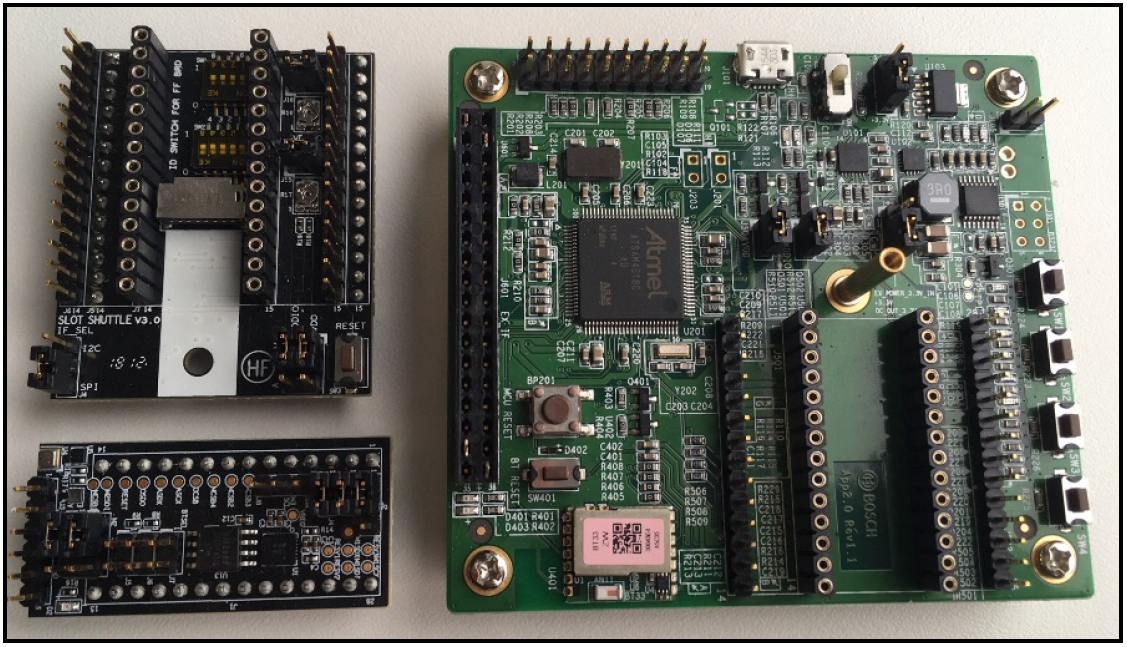
\includegraphics[width=5.5in]{figs/sensor.PNG}}
\caption[BHI260AP Sensor]{BHI260AP Sensor \cite{BoschSensorSetupGuide}}
\label{fig:sensor}
\end{figure}

During the testing of this sensor, three approaches were attempted:

\begin{itemize}
    \item \textbf{Python API}: there was an attempt to use the Python library to communicate with the sensor but although communication was established, there was a lack of documentation and examples that allowed to create code that collected data;
    \item \textbf{C++ API}: there was also an attempt to use the C++ library to communicate with the sensor but the instructions available resulted in a compilation error;
    \item \textbf{Development Desktop 2.0}: this is a desktop application for Windows that allows communication with all Bosch Sensortec sensors and using it, it was possible to collect data to a file or display it in graphs such as in Fig.~\ref{fig:dd2}.
\end{itemize}

\begin{figure}[H]
\centerline{\includegraphics[width=6in]{figs/boschDD2.PNG}}
\caption[Development Desktop 2.0 Interface]{Development Desktop 2.0 Interface \cite{BoschDD2}}
\label{fig:dd2}
\end{figure}

Therefore, collecting data was only possible with the Development Desktop 2.0. However, using the Python or the C++ APIs would be ideal since, as they work in Linux, it would be possible to integrate their usage with \acs{ros}.
